\chapter{Discussion}\label{sec:discussion}
% See http://libguides.usc.edu/writingguide/discussion for how to write a discussion

\todo{rephrase}
This section is divided into three parts. First we will discuss the influence of the research questions. Next we will mention issues we faced and which still remain. The last part of this section is dedicated to the ethical questions this project may involve.

\section{Discussing the research question answers something} \todo{better title}

\section{Issues Faced During Development}
\todo{THIS SECTION WILL BE REMOVED IN FAVOUR OF "Open Issues"}
\todo{check if everything is mentioned in ch5. if this is the case: discard this section, mention ch5 in Open Issues}
Over the course of the project, we came across multiple issues. 
\todo{memory problems}
    
\todo{multiprocessing}
\todo{text encoding}
\todo{python neo4j driver}


\section{Open Issues}\label{sec:Discussion - Open Issues}
Although we managed to handle most of the issues that arose during development, some remain unsolved. However, we believe that with more time, we could have found a solution to most issues. This is especially true for the classifier. Open issues with the classifier are therefore discussed separately, in section \ref{sec:discuss-classifier}.

\todo{subsection titles identical to those in ch5}
\subsection{Downloading and Parsing Indices}
The downloading part of the system is arguably the easiest of all. Indeed, the issues that remain are more related to the resources available, than to the implementation. Downloading speed is dependent on the connection to Common Crawl. Since their data is hosted at Amazon, it might be a lot faster to use a virtual private server of Amazon to host the system on, at least for data collection and storage. One is then able to use the Simple Storage Server (S3)\footnote{\url{https://aws.amazon.com/s3/}} to pull data more quickly from Common Crawl.

Another significant improvement is to use SSD instead of HDD storage, to speed up both reading and writing of files.

A final issue is that Web developers can choose which character set they use for the page content. We were struggling to find a fast and correct way to determine the encoding of the page and then convert it accordingly to a general encoding. Eventually, we decided to stick to UTF-8 for every document and ignore characters that cannot be encoded in UTF-8. However, ISO 8859-1 (also known as latin-1) is widely used in the Netherlands for special characters.

\subsection{Filtering the Data}
Filtering the downloaded documents went quite well overall, as explained in section \ref{sec:5-filtering}. However, we did leave out some important aspects. Most importantly, we had no means of checking on city aliases (like 's-Gravenhage is for Den Haag and Domstad for Utrecht). Additionally, we did not check for complex occurrences of cities, such as "Amsterdammers", people from Amsterdam. We decided to do this due to some large cities that are identical to or contained in commonly used words. An example of this is the city Leiden, which translates directly to the verb "to lead". However, filtering every complex occurrence out is a too aggressive kind of filtering, resulting in discarding otherwise useful documents.

\subsection{Storing the Data}
Storing the data efficiently turned out to be slightly harder than expected due to the many issues we faced. The issues that were overcome are discussed in section \ref{sec: 5-storing}. There are some that have been left open. The most structural issue is that after all, a graph database is a bit overkill for our purposes. We traverse nodes with only a maximum depth of two (for documents in which both city A and city B occur). Such traversals are not complex and might even perform better in a SQL database with foreign keys.

Besides, we did not manage to get the database speed that we expected to reach. This could have to do with the fact that we use the HTTP transactional endpoint instead of the internal API, which is only available for the Java programming language. Perhaps it would have been better to write the database code in Java instead of in Python to use this internal API. It probably has also to do with the fact that we do not have a physical server with a modern SSD at hand to run the database on. This would increase reading and writing speeds significantly.

\subsection{System API}
The most prominent issue with the system API is the lack of authentication and authorisation. This can lead to serious security issues, since anyone can send requests to the API and make the system execute operations. User authentication and authorisation can be added easily\footnote{\url{https://realpython.com/blog/python/token-based-authentication-with-flask/}} but was left out unfortunately due to time constraints.\\
Another issue that is left for the API is that the API does not provide all the functionality that may be wanted in the (near) future. Again this is because of time constraints, which forced us to implement only the routes that were needed for the minimum viable product.\\
\subsection{Front-End}
The main issue in the front end is that settings interface is not connected yet to the API. This means, although we do have the setup for the interface, that submitting a setting from the interface does not trigger a call to the API.\\
Furthermore we have small styling issues. For example relations that have a really small total score are almost invisible when visualised on the map. Fixing this would be done by adjusting the scaling function, which takes the total relations score and scales it to an number between 0 and 1 relative to the maximum total relation score (scaling now is done by applying the square root function to $total\_score/max\_total\_score$).\\
One last issue is the styling of the loaded document in the classification interface. To display the document we load it into a HTML \texttt{<pre>} tag. The HTML \texttt{<pre>} tag displays text like it was formatted, other HTML tags skip white space and line breaks. Since we parse HTML pages to plain text we end up with documents that have a lot of white space and line breaks, which leads to ...., an example is show in figure \ref{fig:ugly-pre}. This can be fixed by pre-processing the do documents before they get loaded into the \texttt{<pre>} tag. This will not harm the validity of the data set since we do not alter any meaningful content.

\begin{figure}[H]
\centering
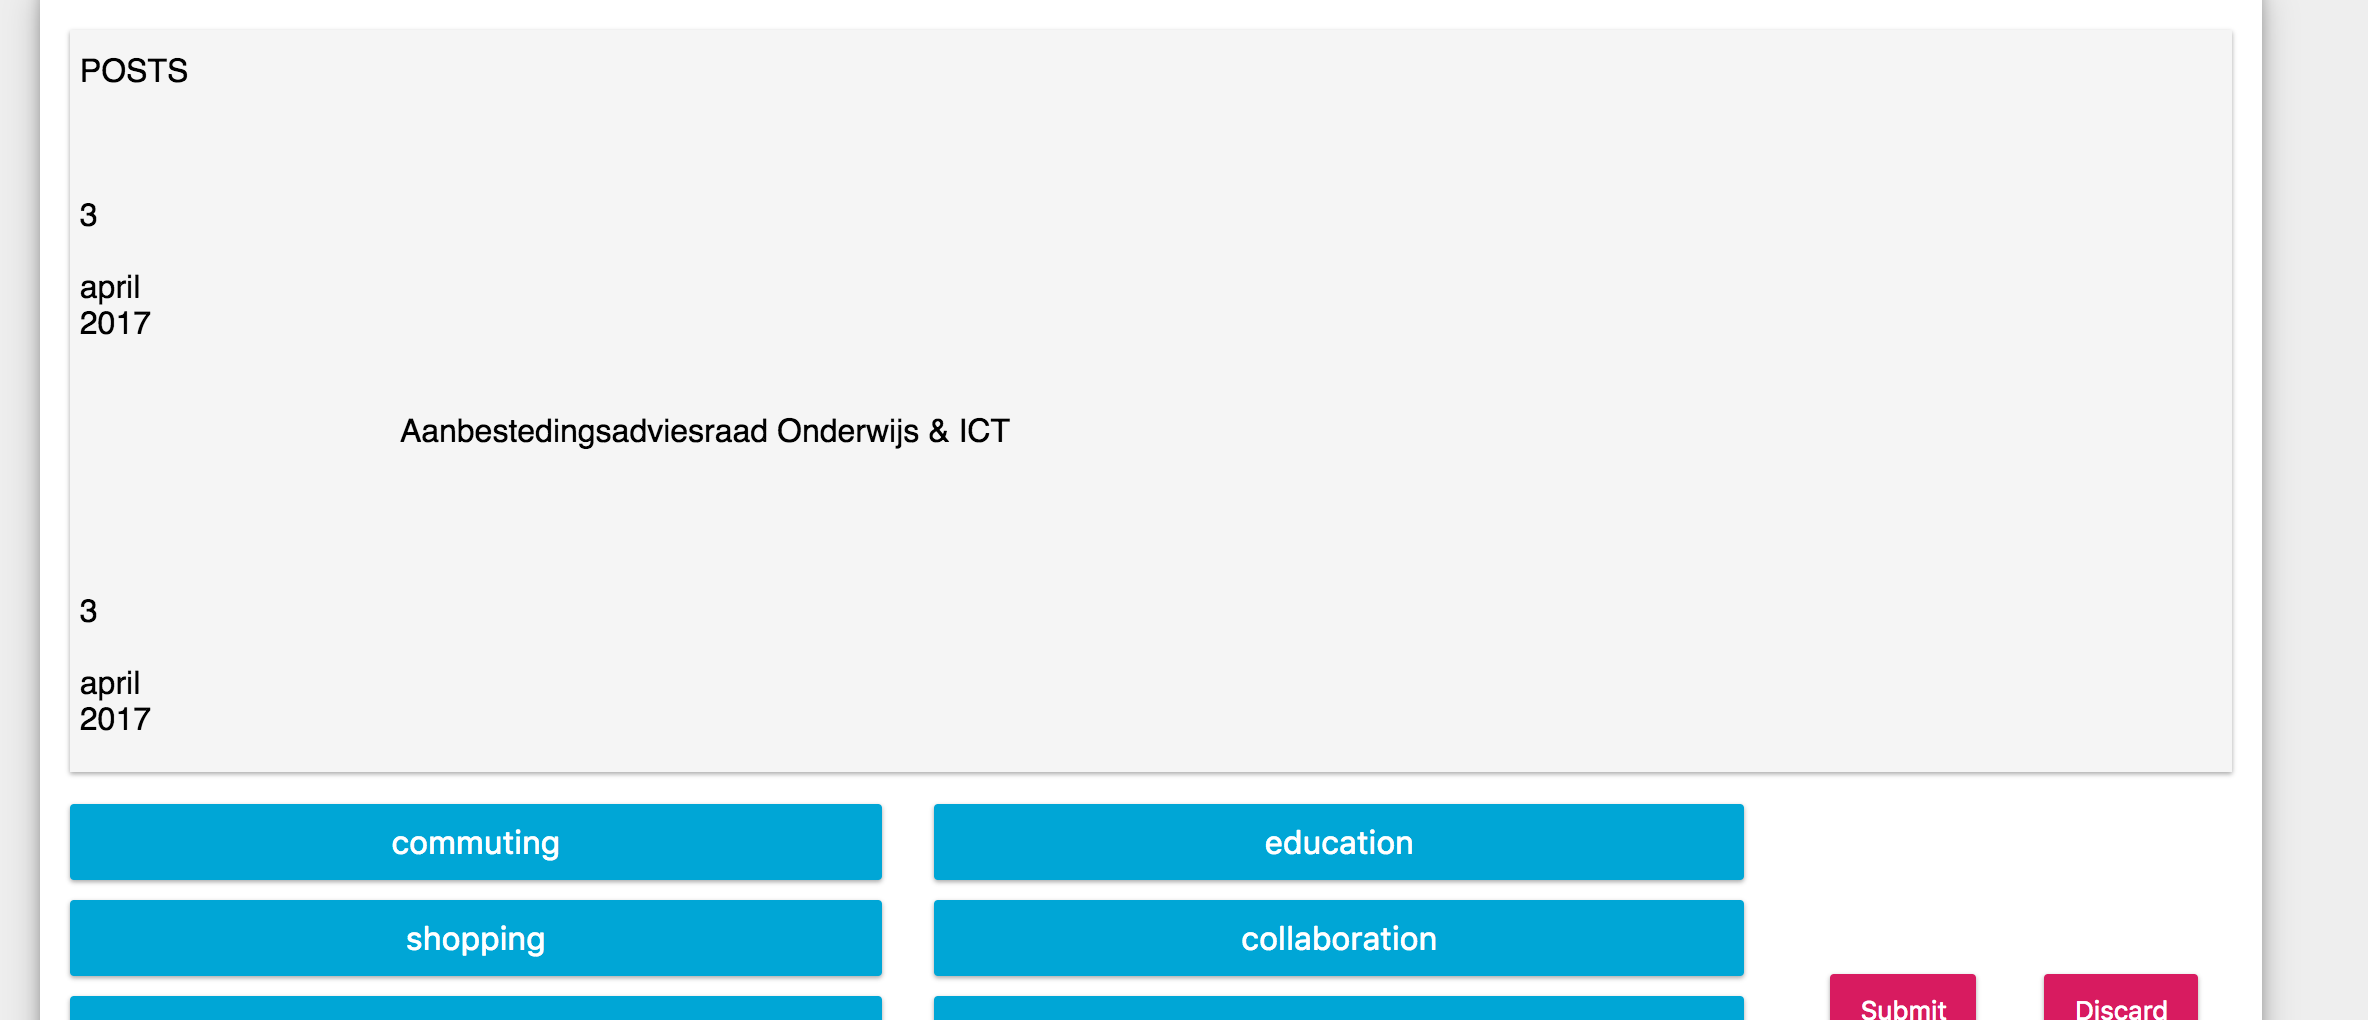
\includegraphics[width=0.6\textwidth]{frontend-ugly-pre}
\caption{Example of an undesired result obtained with Google Custom Search}
\label{fig:ugly-pre}
\end{figure}




\subsection{Main Application}
Combining all components of the system into a full-fledged main application went fine overall. However, a few features were left out that in fact should have been present. For example, there is no decent way for invoking the application via the command line. The code has to be adjusted depending on what part of the system should be started. Moreover, not every part of the system is configurable and we have no progress indication if the system is running. However, we believe these features can be easily added in future versions. It was therefore not our top priority to include them.


% \todo{Discuss choice to filter "Amsterdammers", future version might include this}
% \todo{exporting data}
% \todo{uneven amount of documents/class}
% \todo{language}
% \todo{processing time}
% \todo{neo4j problems}
% \todo{NoSQL vs SQL}
% \todo{more....}

% describe issues faced during implementation, as well as issues that are still 
% open. Main thing here is to discuss the Neo4j python driver with multiprocessing,
% which we could not get to work. Also mention the state of the document 
% classification
\section{Classification} \label{sec:discuss-classifier}
% Describe issues faced during implementation/development
%Discuss open issues 

\section{Ethics}
In this section some of the ethical issues with respect to the developed product are discussed. First, possible issues with storing web data are discussed. Next, we discuss the potential consequences of extracted relations.
%Last, we will look at the environmental impact of running the application and storing the data.

\subsection{Storage of Data}
One of the ethical issues is the storage of web pages. Although these pages are accessible to anyone at the time of downloading, this might change in the future. The owner of the original web page may have good reason to delete the original page, however, this does not mean it is deleted from the local storage of our application. Another issue with storing the web pages locally is a potential violation of copyright. As Thelwall et al. stated, "web crawlers ostensibly do something illegal: They make permanent copies of copyright material (Web pages) without the owner’s permission."\cite{thelwall2006web} Because we store copies of the web data that has been crawled and stored by Common Crawl, the same applies to our application.

\subsection{Consequences of Extracted Relations}
Another issue is that it is unknown how the results of the application will be used. It was designed for research purposes, but there is no way of knowing what the results will be used for. For example, the extracted relationships show which cities are the most important in a network of cities. This information can be used by terrorists to decide to strike in the most important city to maximise the impact. 

The results may also result in some cities becoming more popular, which means they would grow in size. This might have a negative impact on for example the health and living conditions of the people in these cities.

%\subsection{Environmental Impact}
%To run the application and provide the required amount of storage the application will be deployed on one or multiple servers. These servers need to be powered and cooled which means that running the application to parse all the data will have a negative impact on the environment. The question is whether the benefits of having the results of the application outweigh the negative impact it might have on the environment.
